


\ifnumequal{\value{rolldice}}{0}{
  % variables 
  \renewcommand{\va}{-1}
  \renewcommand{\vb}{2}
  \renewcommand{\vc}{1}
  \renewcommand{\vd}{1}
  \renewcommand{\ve}{15}
  \renewcommand{\vf}{6}
  \renewcommand{\vg}{-8}
  \renewcommand{\vh}{11}
  \renewcommand{\vi}{10}
}{
  \ifnumequal{\value{rolldice}}{1}{
    % variables 
    \renewcommand{\va}{2}
    \renewcommand{\vb}{-1}
    \renewcommand{\vc}{1}
    \renewcommand{\vd}{+1}
    \renewcommand{\ve}{15}
    \renewcommand{\vf}{8}
    \renewcommand{\vg}{-6}
    \renewcommand{\vh}{13}
    \renewcommand{\vi}{10}
  }{
    \ifnumequal{\value{rolldice}}{2}{
      % variables 
      \renewcommand{\va}{7}
      \renewcommand{\vb}{2}
      \renewcommand{\vc}{1}
      \renewcommand{\vd}{-1}
      \renewcommand{\ve}{-9}
      \renewcommand{\vf}{3}
      \renewcommand{\vg}{4}
      \renewcommand{\vh}{11}
      \renewcommand{\vi}{10}
    }{
      % variables 
      \renewcommand{\va}{5}
      \renewcommand{\vb}{0}
      \renewcommand{\vc}{1}
      \renewcommand{\vd}{-1}
      \renewcommand{\ve}{-9}
      \renewcommand{\vf}{4}
      \renewcommand{\vg}{3}
      \renewcommand{\vh}{13}
      \renewcommand{\vi}{10}
    }
  }
}

\FRACTIONSIMPLIFY{-\vf}\vg\n\d
\gcalcexpr[0]\c{(\n * \va) - (\d * \vb)}
\SOLVELINEARSYSTEM(\vc,\vd ; \n, -\d)(\ve,\c)(\p,\q)

\question Find the distance of the point $A = (\va, \vb)$ from the line 
$L_1: \gsign\vc x \gsign\vd y = \ve$ measured parallel to the line 
$L_2: \gsign\vf x \gsign\vg y \gsign\vh = 0$.

\watchout

\ifprintanswers
  \vspace{0.3cm}
  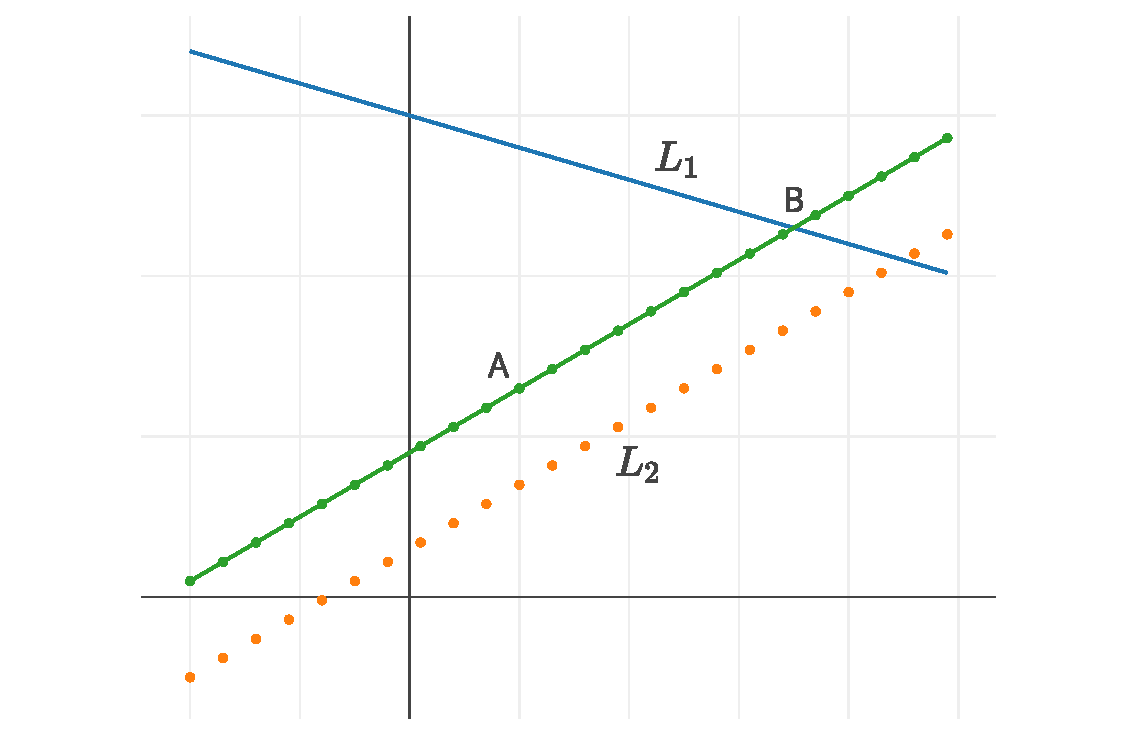
\includegraphics[width=300pt]{plotly.eps}
\fi 

\begin{solution}[\halfpage]
  The situation is as shown in the figure above. 

  There is a point $B$ on line $L_1$ such that $AB\parallel L_2$. We have to find the distance between points $A$ and $B$. 
  
  Now, the point $B = (m,n)$ satisfies the following two conditions
  \begin{align}
  	\gsign\vc m \gsign\vd n &= \ve \because \text{ its on } L_1 \\
  	\dfrac{\vb - n}{\va - m} &= \dfrac{\n}{\d} \because AB \parallel L_2 \\
  	\implies \n m - \d n &= \c
  \end{align}
  Solving (1) and (3), we get $B = (m,n) = (\p,\q)$. 
  
  Now we know everything to calculate the distance 
  between $A$ and $B$
  \begin{align}
    D &= \sqrt{(\p - \va)^2 + (\q - \vb)^2} = \vi\text{ units.}
  \end{align}
\end{solution}

\ifprintanswers\begin{codex}$\vi\text{ units}$\end{codex}\fi
